% !TeX root = ../main.tex
% Add the above to each chapter to make compiling the PDF easier in some editors.

\chapter{Introduction}\label{chapter:introduction}

The goal of this thesis is to obtain an implementation of B-Trees in the Isabelle/HOL Framework.
The approach is to first design a functional, abstract implementation.
This implementation is the shown to implement a Set-interface,
correctly implementing retrieval, insertion and deletion operations.
In a last step, an imperative implementation is derived that
refines the functional variant.
Thus the proof of correctness for the imperative implementation
is reduced to a proof of equivalence between the output of the
functional and the imperative implementation.
Desirable properties regarding low runtime and high storage usage
are preserved by the obtained implementation.

% TODO related work?

\section{The Isabelle Proof Assistant}

Isabelle/HOL is an interactive theorem prover.
It is built on PolyML, a functional language similar to OCaml
and Haskell.% TODO factual accuracy
The implementation will hence make use of newly defined functions, where
\texttt{definition} denotes classical definitions and \texttt{fun} (an abbreviation of "function")
is used for recursive definitions.
Definitions that are not explicitly denoted with \texttt{partial\_fun}
incorporate an automatic proof of termination.

Theorems can be formulated in a similar manner to how they written in this paper.
To prove a theorem correct, the system basically provides two different
proof styles.
In the apply-Style, the user tells the system which proof method
to apply to modify the current goal.
This is practical if the number of assumptions
is high or the goal is large and writing the terms
out would be impractical.
Since this is the case for the proofs of the imperative programs,
almost all proofs in \autoref{chapter:imp-set} are written in this style.

The other option is to write structured proofs.
The user outlines a proof with intermediate goals
and tells the system which proof methods to apply to
resolve each step.
This method is usually preferred as it is more readable and usually
faster on the system side.
All complex proofs in \autoref{chapter:abs-set} are hence written in this style.

The system provides a number of proof methods,
such as logical or set reasoning or simplification.
When talking about "automatic" proofs, usually a proof that follows
by applying a single command is meant (such as the method \texttt{auto},
a combination of logical reasoning and simplification).

Datatypes may be defined recursively.
The following shows as an example the internal definition of the list datatype.\footnote{
    The actual definition is worded slightly different but this is of no importance here.
}

\begin{lstlisting}[mathescape=true, language=Isabelle,label=lst:list-def]
datatype 'a list = [] | 'a # 'a list
\end{lstlisting}

In natural language this means that either a list is the empty list,
or it is an element prepended on another list.
As usual in ML like languages, we may deconstruct an argument to a function
by pattern matching to this construction.
In addition, the type $'t$ of any expression $e$ can be
made explicit by writing \textit{e :: 't}.
Functions that take values of type $'a$ and return values of type $'b$ 
have type \textit{'a $\Rightarrow$ 'b}.
The Isabelle internal list catenation function serves as
an example for a function definition with explicit type.

\begin{lstlisting}[mathescape=true, language=Isabelle,label=lst:append-def]
fun (@) :: 'a list $\Rightarrow$ 'a list $\Rightarrow$ 'a list where
    [] @ ys = ys |
    (x#xs) @ ys = x # (xs @ ys)
\end{lstlisting}

Further details on notation, proof techniques and more in Isabelle/HOL
may be found in \parencite{DBLP:books/sp/NipkowPW02}.

% function notation (like haskell/OCaml)
% NOTE all functions terminate, unless declared "partial"
% can write mathematical expressions (?)
% list notation etc
% proof styles, methods (?)
% locales
% set specification
% TODO cite isabelle resources

\section{The B-Tree Data Structure}

B-Trees were first proposed by Bayer et al. in \parencite{DBLP:journals/acta/BayerM72},
as a data-structure to efficiently store and retrieve indices stored on storage devices
with slow memory access.
% TODO reorder with definitions
They are a generalization of 234-Trees and a specialization of (a,b)-Trees
%TODO citation
and as such hence a kind of balanced search-trees.
The number of subtrees in each node is defined by the \textit{order} $k$ of the tree.

\subsection{Definitions}
\label{sec:data_structure_defs}

Every node contains a list of \texttt{keys} or \texttt{separators}, index elements, and \texttt{subtrees},
that refer to further B-Trees.
The length of this list is bounded by \texttt{k}.
The separators and subtrees are considered interleaved within a node,
such that we can speak of a subtree left of a separator and a subtree right of a separator,
where for a separator at index \texttt{i} we mean the subtree in the respective
subtree list at index \texttt{i} and \texttt{i+1} respectively.
Note that this already implies that the list of subtrees is one
longer than the list of separators - we refer to the last subtree as the \textit{last} or
\textit{dangling} subtree.
In \parencite{DBLP:journals/acta/BayerM72},
a B-Tree with above structure must fulfill the three properties
\textit{balancedness}, \textit{order} and \textit{sortedness}.

\textit{Balancedness} requires that each path from the root to any leaf has the same length \texttt{h},
in other words that the height of all trees in one level of the tree must be equal.

Further the indices must be \textit{sorted} within the tree which means that all indices stored
in the subtree left of a separator are smaller than the value of the separator
and all indices on the right are greater.

In general terms, the property of \textit{order} ensures a certain minimum and maximum
number of subtrees for each node.
However, as pointed out in \parencite{DBLP:books/daglib/0095349_mod},
the property is defined differently in the literature.
For the purpose of this work, the original definition by Bayer et al. was chosen as most suitable.
A B-Tree is of order $k$, if each internal node has at least $k+1$
subtrees and at most $2k+1$.
The alternative of defining the nodes to have between $\lceil \frac{k}{2} \rceil$
and $k$ children (as proposed in \parencite{DBLP:books/lib/Knuth98a}),
involves cumbersome \textit{real} arithmetic that unnecessarily complicates
mechanized proofs.
Sticking to the original definition is further supported by the fact that nodes are supposed
to fill memory pages which are usually of even size (usually some power of 2).
An even number of separators and trees plus one dangling last right tree maximizes
the usage of such a page.

The same ambiguity exists for the term \textit{Leaf} which we will define consistently with Knuth's definition \parencite{DBLP:books/lib/Knuth98a}
to be an empty node, carrying no information.
This is closest to the usual approach in functional programming.
The lowest level of nodes hence contains a list of separators and
list of pointers to leaves.

% TODO insert image of valid B-Tree
A simple B-Tree may be seen in \autoref{fig:btree-basic-nopair}
\begin{figure}
    \centering
    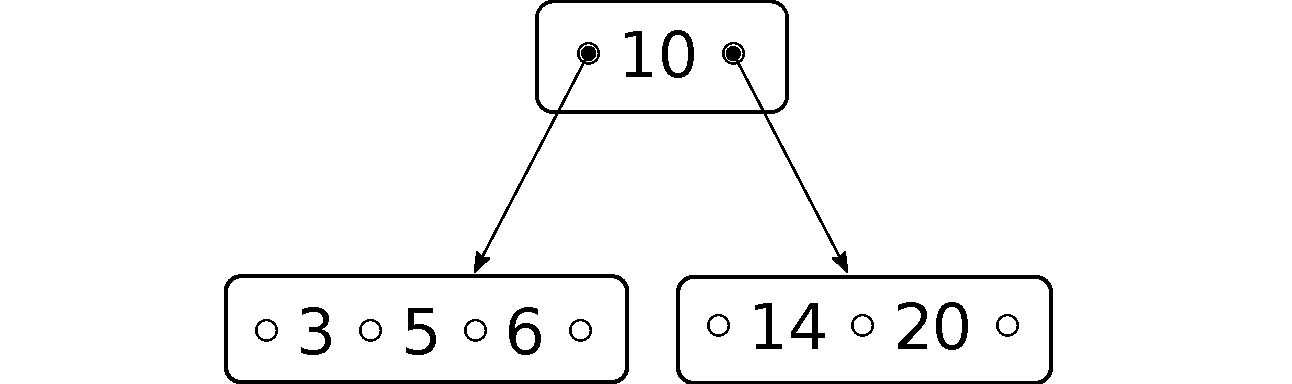
\includegraphics[width=0.5\linewidth]{figures/btree-basic-nopair.pdf}
    \caption{A small balanced B-Tree of order $2$ and
    height $2$ containing $3$ nodes and $6$ elements.}
    \label{fig:btree-basic-nopair}
\end{figure}

\subsection{Desirable Properties}

B-Trees are assumed to be stored on external memory,
such that each node roughly matches a page in main memory.
Due to the potentially large branching factor and the balancing,
the number of required memory accesses for retrieving data stays small even for
large amounts of data stored.
This is due to the fact that the overall number of memory accesses is bounded by the depth
of the tree, which again is logarithmic in the number of indices -
where the base of the logarithm is closely proportional to the order $k$ of the tree.

Further, by design, the storage usage of B-Trees is at a minimum close to $50\%$,
where the average usage is usually higher. \parencite{DBLP:journals/acta/BayerM72}
This is due to the fact that every node reserves the storage of $2k$ keys and separators
but by definition always contains at least $k$ elements.

These properties are key to the widespread popularity of B-Trees and are
hence preserved in the given implementation.


\subsection{Applications}

B-Trees are used in almost all modern databases for storing key-value pairs.
% TODO more

\chapter{Functional B-Trees in Isabelle}\label{chapter:abs-set}

Functional specifications of data structures tend to have properties that
are easier to prove than for corresponding imperative implementations
mostly due to the fact that many details of implementation can be abstracted away.
The work therefore begins with a functional specification of B-Trees.

\section{Basic Definitions}
\label{sec:basic-defs}
%Definition used for this implementation.
%(esp. order)
%note that k refers to keys+subtrees rather than only keys/subtrees (false! we have k pairs)

% TODO all function equations similar to math equations, setting variables in italics

Inspired by the design in \parencite{DBLP:conf/popl/MalechaMSW10}, the B-Tree data-structure is defined as follows:

\begin{lstlisting}[mathescape=true, language=Isabelle,label=lst:btree-def]
datatype 'a btree = Leaf | Node ( 'a btree * 'a ) list 'a btree
\end{lstlisting}

\begin{figure}
    \centering
    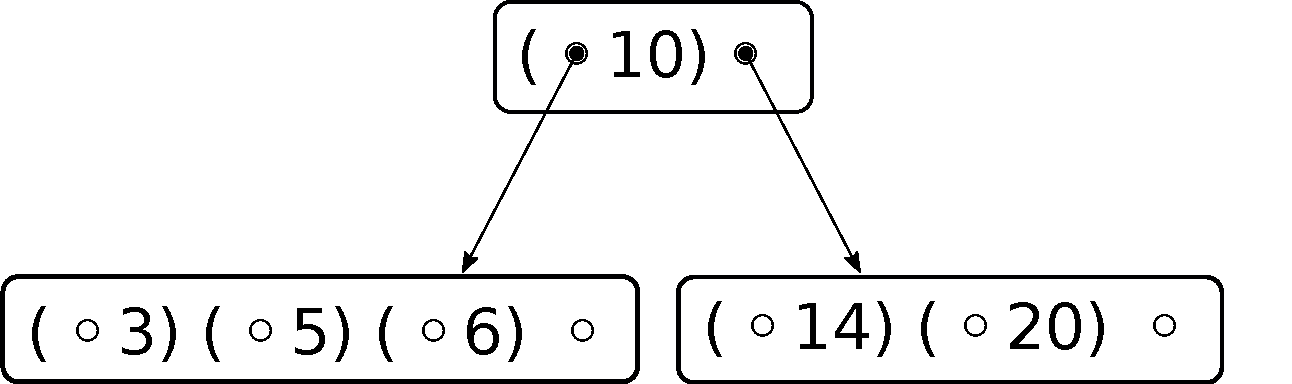
\includegraphics[width=0.5\linewidth]{figures/btree-basic.pdf}
    \caption{The B-Tree from figure \autoref{fig:btree-basic-nopair}.
    Subtrees and separators that lie in pairs in the implementation are surrounded by brackets.}
    \label{fig:btree-basic}
\end{figure}

By interleaving the subtrees and separators, expression of invariants
on the tree is possible without the explicit use of indices into lists.
Since the list of trees is exactly one longer than the list of keys,
the last tree is added to the node in a special position.
The construction leads to the fact that it is easiest to relate any separator
to the subtree on the left, as this subtree is in the same tuple.
Operations that require the subtree on the right can always be expressed as a special
operation on the last tree.

The balancedness of a B-Tree is defined in a straightforward fashion, making use
of an intuitively defined height.\footnote{
    Note that the actual implementation of height is slightly different,
    however this is of no importance in any proofs but rather notationally convenient.
}
There is a choice here, namely whether to fix the balancedness of a tree
on some arbitrary number or on a known value.
Since we know the last tree in the node exists and further
know that all in the node have the same height as that tree,
we simply choose the height of the last tree as an anchor point.

\begin{lstlisting}[mathescape=true, language=Isabelle]

fun height :: 'a btree $\Rightarrow$ nat where
  height Leaf = 0 |
  height (Node ts t) = 1 + (fold max (map height (subtrees ts)) (height t))

fun bal :: 'a btree $\Rightarrow$ bool where
    bal Leaf = True |
    bal (Node ts t) = (
      ($\forall$sub $\in$ set (subtrees ts). height t = height sub) $\wedge$
      ($\forall$sub $\in$ set (subtrees ts). bal sub) $\wedge$
      bal t
    )
\end{lstlisting}

Further the \textit{order} of the trees needs to be formally defined.
As discussed in \autoref{sec:data_structure_defs}, the most useful choice here is
to allow for at least $k$ and at most $2*k+1$ subtrees.
Since the last subtree is fixed, this means that the length of list of keys and children
itself has to be between $k$ and $2*k$.
Note that we also need a special property $order^r$ for the root of the tree,
which has between one and $2*k$ elements.
In mathematical equations, we will denote "order $k$ $t$" as "$\order_k t$"
for convenience (likewise for "order$^r$ $k$ $t$"), which is to be read as
"Tree $t$ is of order $k$".

\begin{lstlisting}[mathescape=true, language=Isabelle]

fun order :: nat $\Rightarrow$ 'a btree $\Rightarrow$ bool where
    order k Leaf = True |
    order k (Node ts t) = (
    (length ts $\ge$ k)  $\wedge$
    (length ts $\le$ 2*k) $\wedge$
    ($\forall$sub $\in$ set (subtrees ts). order k sub) $\wedge$
    order k t
  )

fun order$^r$ where
  order$^r$ k Leaf = True |
  order$^r$ k (Node ts t) = (
  (length ts $>$ 0) $\wedge$
  (length ts $\le$ 2*k) $\wedge$
  ($\forall$s $\in$ set (subtrees ts). order k s) $\wedge$
   order k t
)

\end{lstlisting}

We define the sortedness of a B-Tree based on the \textit{inorder} of the tree,
which is the concatenation of all elements of the tree in in-order traversal.
A concatenation function for lists of strings
is employed to express the resulting string,
since each node does no longer have a constant maximum number of elements (as opposed to
e.g. 2-3-4-Trees in \parencite{DBLP:conf/itp/Nipkow16}),
Note that this definition reads a bit inconveniently
as the node internal list is first mapped and then concatenated.
However since we make recursive use of the inorder-function
inside the mapping expression, we can only later on cover up this expression
by using abbreviations.
In mathematical terms in the following, we will not distinguish between lists, 
pairs or trees when talking about their inorder representation.

\begin{lstlisting}[mathescape=true, language=Isabelle]
fun inorder :: 'a btree $\Rightarrow$ 'a list where
    inorder Leaf = [] |
    inorder (Node ts t) = 
        concat (map ($\lambda$ (sub, sep). inorder sub @ [sep]) ts)
        @ inorder t

abbreviation inorder_pair  $\equiv$ $\lambda$(sub,sep). inorder sub @ [sep]
abbreviation inorder_list ts $\equiv$ concat (map inorder_pair ts)
\end{lstlisting}

That way we can express sortedness of the tree $t$ as a simple $\sorted (\inorder t)$,
where sorted returns whether each element is strictly smaller ($<$) than the elements in the remaining list.
This definition is very compact and brings for another benefit pointed out by Nipkow et al in \parencite{DBLP:conf/itp/Nipkow16}.
Many properties of B-Trees follow intuitively by considering
the inorder view on the tree as it is invariant for many operations (i.e. stealing from the right neighbor node).
We will see later how the use of this fact comes in handy for proving
important properties of the implementation.

Since B-Trees are usually only defined for positive
orders, we obtain the following overall invariant for B-Trees.
\begin{definition}
    $k > 0 \Longrightarrow \btree_k t := \bal t \wedge \order^r_k t \wedge \sorted (\inorder t)$
\end{definition}

The B-Tree definition is only meaningful for positive $k$.
For the case that $k$ is equal to 0,
all elements of the tree would have exactly one subtree
and no internal elements.
For the root node this even leads to a contradictory state:
It is required to contain at least 1 element.
However as it should not have more than $2k=0$ elements,
this constraint cannot be satisfied.
This is consistent with the common definitions.
 % TODO note benefit over btree_sorted

\section{Height of B-Trees}

%Height etc.
As pointed out by Bayer in the first paper describing B-Trees,
the height of B-Trees is logarithmic with respect to the number
of nodes of the tree. \parencite{DBLP:journals/acta/BayerM72}
The paper even gives a precise lower and upper bound, which will be quickly sketched in the following.

First, we define the number of nodes in a tree:
\begin{lstlisting}[mathescape=true, language=Isabelle]
fun nodes :: 'a btree $\Rightarrow$ nat where
    nodes Leaf = 0 |
    nodes (Node ts t) =
        1 + $\sum$t$\leftarrow$subtrees ts. nodes t + nodes t
\end{lstlisting}

%To work with this equation, we just need to add one auxiliary lemmas to the standard canon
%\begin{lemma}
%\begin{lstlisting}[mathescape=true, language=Isabelle]
%    sum_list (replicate n c) = n*c
%\end{lstlisting}
%\end{lemma}

We obtain bounds
on the number of nodes of an subtree with respect to its height
by induction on the computation of the nodes function.

\begin{lemma}
    \label{lem:bound_internal_node}
    $\order_k t \wedge \bal t \longrightarrow$
    \begin{align}
        (k+1)^{\height t} - 1 &\le \nodes t * k \\
        \nodes t * 2k &\le (2k+1)^{\height t} - 1
    \end{align}
\end{lemma}

From \autoref{lem:bound_internal_node} we can almost directly obtain
the bounds on valid roots of B-Trees.
The only difference to the bound of internal nodes occurs on the lower bound side.
The issue here is that a root node may contain less elements than
a valid internal node (namely only one), which yields two subtrees with known height
plus one for the node itself.
Note that these are the exact bounds obtained by Bayer et al. in \parencite{DBLP:journals/acta/BayerM72},
except for the fact that we have generalized the equation,
incorporating whether $t$ is a tree or not.\footnote{
    If $t$ is in fact a Leaf,
    $2((k+1)^{\height t - 1} - 1) \div k + (t \neq Leaf)$ becomes a fancy way of writing $0$.
}

\begin{theorem}
    $\rootorder_k t \wedge \bal t \wedge k > 0 \longrightarrow$
    \begin{equation}
        2((k+1)^{\height t - 1} - 1) \div k + (t \neq Leaf) \le \nodes t \le ((2k+1)^{\height t} - 1) \div 2k
    \end{equation}
\end{theorem}

These results are very interesting, because
the runtime of all further operations will more or less trivially be
directly proportional to the height of the tree.
Therefore, we are glad to see that the height is logarithmic
with respect to the number of nodes stored in the tree.

These bounds are sharp, which we prove by providing 
functions that generate exactly those trees
that satisfy the requirements of B-Trees, have a given height
and satisfy the inequality with equality (in \autoref{lst:sharp-trees-def})
The proof for internal nodes follows by induction over the creation,
the rule for the roots follows directly.

\begin{figure}
\begin{lstlisting}[mathescape=true, language=Isabelle,label={lst:sharp-trees-def},
    caption={The functions generating trees with minimal size and maximal size for given height.}]

fun full_node where
  full_node k c 0 = Leaf |
  full_node k c (Suc n) = (
      Node
        (replicate (2*k) ((full_node k c n),c))
        (full_node k c n)
  )

fun slim_node where
  slim_node k c 0 = Leaf |
  slim_node k c (Suc n) = (
      Node
        (replicate k ((slim_node k c n),c))
        (slim_node k c n)
    )

definition full_tree = full_node

fun slim_tree where
  slim_tree k c 0 = Leaf |
  slim_tree k c (Suc h) =
    Node
        [(slim_node k c h, c)]
        (slim_node k c h)

\end{lstlisting}
\end{figure}

%TODO (?) images of slim/full trees

\begin{lemma} $t_f := \fullnode k\ a\ h \wedge t_s := \slimnode k\ a\ h \longrightarrow$
    \begin{align}
    h = \height t_s = \height t_f \wedge \\
    ((2k+1)^h - 1) &= \nodes t_f * (2k) &\wedge \order_k t_f \wedge \bal t_f \\ 
    ((k+1)^h - 1) &= \nodes t_s * k  &\wedge \order_k t_s \wedge \bal t_s
    \end{align}
\end{lemma}

% TODO prove div version of thm
\begin{theorem}
    $k > 0 \wedge t_f := \fulltree k\ a\ h \wedge t_s := \slimtree k\ a\ h \longrightarrow$
    \begin{align}
    h = \height t_s = \height t_f \wedge \\
        ((2k+1)^h - 1) \div 2k &= \nodes t_f &\wedge \rootorder_k t_f \wedge \bal t_f \\ 
        2((k+1)^h - 1) \div k + (t_s \neq Leaf) &= \nodes t_s &\wedge \rootorder_k t_s \wedge \bal t_s
    \end{align}
\end{theorem}


\section{Set operations}

With the definition of B-Trees come a number of operations that allow for set-like operations
on the trees - retrieval, insertion and deletion.
In the Isabelle/HOL framework, there is a standard interface
for data structures that provide an implementation of sets.

\subsection{The Set Interface}
% Description of the set interface

An implementation $'a t$ of the sets of elements of type $'a$ is required to provide the following
operations

\begin{itemize}
    \itshape
    \item empty :: 'a t
    \item isin :: 'a t $\Rightarrow$ 'a $\Rightarrow$ bool
    \item insert :: 'a $\Rightarrow$ 'a t $\Rightarrow$ 'a t
    \item delete :: 'a $\Rightarrow$ 'a t $\Rightarrow$ 'a t
\end{itemize}

In addition an \textit{invariant :: 'a t $\Rightarrow$ bool} has to be supplied
that stays unchanged by all operations.
For this work, using the definition from \autoref{lst:btree-def},
we consider \textit{'a t = 'a btree} in all above equations.
The standard approach is to show that we can provide functions for the B-Tree
that have the same effect as insertion, deletion or testing on contained elements
in abstract sets with the same elements.

We know from \autoref{sec:basic-defs} that one of the invariants
of the tree is that it is always sorted.
While this is expressed in a somewhat cumbersome manner
in the original definition \parencite{DBLP:journals/acta/BayerM72},
this requirement is nothing else but a sortedness of the inorder view of the tree.
Knowing this, we resort to a specialized Set interface
proposed in \parencite{DBLP:conf/itp/Nipkow16}.
In that work, the approach yielded automatic proofs for 2-3-Trees
and 2-3-4-Trees, which are specializations of B-Trees.

The invariant and inorder functions for this set interface
follow directly from the definition of B-Trees in \autoref{sec:basic-defs}.
Hence, we specify $k > 0 \wedge \order^r_k t \wedge \bal t$
as the invariant of B-Trees.
The interface is then implemented by providing set operations
and the proofs of invariant preservation.

Some parts of the Set specification are trivial.
In the following, \textit{Leaf} is an empty tree and hence represents
the empty set, satisfying the first part of the specification.
It can be seen directly that the leafs already satisfy all three properties.
The following sections will describe the implementation of the
non-trivial set operations.

\subsection{The split-Function}
% Description of the implementation of the set interface.

Naturally the set operations are defined recursively on the nodes of the tree.
Since each node contains a non-trivial number of elements,
a function to navigate to the correct separator and subtree is central to all operations.

We call this function \textit{split}-function,
determining the position in the list of separators and subtrees at which
either the separator is equal to the desired value or the range of the left subtree
contains the desired value.
Since the whole tree is sorted, we know that if the element being searched for
is contained anywhere in the tree, it must be in that subtree.
This approach is similar to the one found in the work of Malecha and Fielding \parencite{DBLP:conf/popl/MalechaMSW10,Fielding80}.\footnote{
    In Fieldings approach the corresponding function is called \textit{index}.
    Malecha calls it \textit{findSubtree}.
}
Usually however, it is integrated into the set-operation
by a linear search that is promised to be replaced by a more efficient binary search
in the actual implementation \parencite{DBLP:books/daglib/0023376,DBLP:journals/acta/BayerM72}
or left in the final code \parencite{DBLP:journals/sosym/ErnstSR15}

The precise inner workings of the split function are not of interest here
and actually are not supposed to be interesting on the functional level.
Of course \textit{some} kind of function is required that correctly splits
the key-value list and an example is given in \autoref{fig:linear_split}.
In the process of implementing the set specifications,
this concrete function was used to explore the provability of the set methods.
However it quickly turned out that 1) only specific lemmas about the split
function are useful during proofs and 2) only relying on an abstract specification of
the split method would simplify integrating alternative splitting functions.
Most notably, the abstraction allows to later plug-in a very efficient splitting
function, e.g. based on binary search.

\begin{figure}
    
\begin{lstlisting}[mathescape=true, language=Isabelle]
fun linear_split_help where
  linear_split_help [] x prev = (prev, []) |
  linear_split_help ((sub, sep)#xs) x prev = (
      if sep < x then
        linear_split_help xs x (prev @ [(sub, sep)])
      else
        (prev, (sub,sep)#xs)
  )

fun linear_split:: ('a btree$\times$'a) list $\Rightarrow$ 'a $\Rightarrow$ (_ list $\times$ _ list) where
  linear_split xs x = linear_split_help xs x []
\end{lstlisting}
\caption{A function implementing the split function specifications.
It scans linearly through the list, returning the first tuple where the separator
or subtree could potentially contain the value $x$}
\label{fig:linear_split}

\end{figure}

Therefore all set functions are defined based the following requirements:

\begin{itemize}
    \item $\splitfun xs\ p = (ls,rs) \Longrightarrow xs = ls @ rs$
    \item $\splitfun xs\ p = (ls@[(sub,sep)],rs) \wedge \sorted (\separators xs) \Longrightarrow sep < p$
    \item $\splitfun xs\ p = (ls,(sub,sep)\#rs) \wedge \sorted (\separators xs) \Longrightarrow p \le sep$
\end{itemize}

Described in natural language, the split function should return two sublists
that concatenate to the original list.
Further if the elements came in sorted order,
the list is split such that the key to the left is strictly less than the desired value
and the key to the right should be less or equal.

The benefit of restricting the sortedness of the list only to its separators
simplifies the proofs of showing that a certain function fulfils the split abstraction.
We really only need to consider the separators on each level and not the subtrees themselves.
Showing that the function works on a sorted inorder list
would only introduce an additional step to follow that the separators are sorted as well.
Having fixated this abstraction we only need to follow this fact once
and can relieve the writer of split functions of the need to do so.

The abstraction was formulated in a locale.
Inside the locale we have access to exactly the specified split function,
without knowing anything about the composition of that function.

\subsection{The $isin$ operation}

%-------------------------------------------------
% TODO move to abstract description?
The simplest operation required in the Set interface is
the \textit{isin} function.
% Note reference to i.e. Bauer retrieval algorithm
The definition in \autoref{lst:isin-fun} also shows exemplary usage of the split function.
In case the right part of the split list is non-empty,
we check the element at that level or recurse in the given subtree.
Otherwise, we may directly recurse to the last tree in the node.\footnote{
    Since this function recurses on the split function,
    in order to show that this function terminates, we need to tell
    the system that the obtained subtrees are of smaller size than the current tree.
    Adding this fact to the default termination simplification set resolves
    the issue for all coming functions.
}
%-------------------------------------------------

\begin{figure}
\begin{lstlisting}[mathescape=true, language=Isabelle, caption=The \textit{isin} function, label=lst:isin-fun]
fun isin:: 'a btree $\Rightarrow$ 'a $\Rightarrow$ bool where
    isin (Leaf) y = False |
    isin (Node ts t) y = (
        case split ts y of (_,(sub,sep)#rs) $\Rightarrow$ (
            if y = sep then
                True
            else
                isin sub y
        )
    | (_,[]) $\Rightarrow$ isin t y
    )
\end{lstlisting}
\end{figure}

By the standard set interface the operation is only required to work on
sorted, balanced trees of a certain order, however only the first property
is actually required for correctness.
The following lemma shows the required property of the function

\begin{theorem}
    \label{thm:isin-set}
    $\sorted (\inorder t) \Longrightarrow \isinfun t\ x = (x \in \setfun (\inorder t))$
\end{theorem}

It follows by induction on the evaluation of the isin function.
To prove it, we invoke two specialized lemmas,
that simplify arguments about the choice of the node for recursion.
The kind of lemmas are of special interest as they specialize
an idea proposed in \parencite{DBLP:conf/itp/Nipkow16} and similar lemmas
are used for the correctness proofs of insert and delete alike.

\begin{lemma}
    $\sorted (\inorder (Node\ ts\ t) \wedge \splitfun ts\ x = (ls, rs) \Longrightarrow$ \\
    $x \in (\setfun (\inorder (Node\ ts\ t))) = (x \in \setfun (\inorder rs @ \inorder t))$
\end{lemma}

The idea of this fact is to argue that, if the split function has provided
us with a given splitting, it is safe to limit the further search
to the right side of the split.
It follows directly from the requirements on the split function.
If $rs$ is empty, we can follow that the element has to reside in the inorder
of the last tree of the node.
When used in the inductive proof of \autoref{thm:isin-set}, we can then deduce that this is
equal to $\isinfun t\ x$, the branch taken in the isin-function (see \autoref{lst:isin-fun}) for an empty right split result.
If $rs$ is not empty, we need an additional lemma.

\begin{lemma}
    $\sorted (\inorder (Node\ ts\ t)) \wedge \splitfun ts\ x = (ls, (sub,sep)\#rs) \wedge sep \neq x \Longrightarrow$ \\
    $x \in (\setfun (\inorder ((sub,sep)\#rs) @ \inorder t)) = (x \in \setfun (\inorder sub))$
\end{lemma}

With this lemma we know that the first subtree on the right part of the split
is the correct child to recurse into.
The requirement of $sep \neq x$ comes from the fact that in case $sep = x$,
no recursion is required at all.
The desired element was just found.

This operation has no effect on the tree, it only walks through it.
This fact follows directly due to the persistence of functional data structures.
Hence, no proof of preserved invariant is required.

\subsection{Insertion}

% TODO move abstract discussion to introduction
%-------------------------------------------------
However this is not true for the \textit{insertion} function.
There is much consensus in the literature on how to conduct insertion into a B-Tree.
%TODO citations
There are not many provably correct functional implementations to our knowledge.
However there is a relationship between 234-Trees and B-Trees,
due to which the approach to the functional definition is inspired by the implementation
in \parencite{DBLP:conf/itp/Nipkow16}.
In that work, a correct implementation of the Set interface for 234-Trees 
are provided.

%TODO relationship to other implementations (are there more?)
Generally, an element is inserted into leaf nodes.
In case that there is enough space left, the element is simply placed at the correct
position in the list of separators.
However if the node has more than $2k$ elements after this insertion,
we need to split it and, passing the median to the parent node,
recurse back upwards.
%-------------------------------------------------

The implementation of the insertion function is documented in \autoref{lst:ins-fun}.
To modularize insertion, the check for the overflow of a nodes list has been
extracted to a function $node_i$.
The function returns data in a new datatype called $up_i$, which
carries either a singleton valid B-Tree or two trees and a separator
that could correctly be part of a node when placed next to each other.
This construction appears the same way in \parencite{DBLP:conf/itp/Nipkow16}.

The $ins$ function is a recursive helper function,
that recurses down into the correct leaf node for inserting the desired element,
and, on the way up, inserts potentially newly obtained subtrees into the
current nodes list with the help of $node_i$.
The $ins$ function also makes use of the new datatype $up_i$ to indicate whether
the current node had an overflow or not.

Finally, the $insert$ function calls the $ins$ helper function
and transforms the result into a valid B-Tree.

\begin{figure}
    
\begin{lstlisting}[mathescape=true, language=Isabelle, label=lst:ins-fun, caption={
    The \textit{insert} function
}]
datatype 'b up$_i$ = T$_i$ 'b btree | Up$_i$ 'b btree 'b 'b btree

fun split_half where
  split_half xs = (take (length xs div 2) xs, drop (length xs div 2) xs)

fun node$_i$:: nat $\Rightarrow$ ('a btree $\times$ 'a) list $\Rightarrow$ 'a btree $\Rightarrow$ 'a up$_i$ where
  node$_i$ k ts t = (
  if length ts $\le$ 2*k then T$_i$ (Node ts t)
  else (
    case split_half ts of (ls, (sub,sep)#rs) $\Rightarrow$
      Up$_i$ (Node ls sub) sep (Node rs t)
    )
  )

fun ins:: nat $\Rightarrow$ 'a $\Rightarrow$ 'a btree $\Rightarrow$ 'a up$_i$ where
  ins k x Leaf = (Up$_i$ Leaf x Leaf) |
  ins k x (Node ts t) = (
  case split ts x of
    (ls,(sub,sep)#rs) $\Rightarrow$ 
      (if sep = x then T$_i$ (Node ts t)
      else
        (case ins k x sub of 
          Up$_i$ l a r $\Rightarrow$
            node$_i$ k (ls @ (l,a)#(r,sep)#rs) t | 
          T$_i$ a $\Rightarrow$ T$_i$ (Node (ls @ (a,sep) # rs) t))) |
    (ls, []) $\Rightarrow$
      (case ins k x t of
         Up$_i$ l a r $\Rightarrow$
            node$_i$ k (ls@[(l,a)]) r |
         T$_i$ a $\Rightarrow$ T$_i$ (Node ls a)
  )
)

fun tree$_i$::'a up$_i$ $\Rightarrow$ 'a btree where
  tree$_i$ (T$_i$ sub) = sub |
  tree$_i$ (Up$_i$ l a r) = (Node [(l,a)] r)

fun insert::nat $\Rightarrow$ 'a $\Rightarrow$ 'a btree $\Rightarrow$ 'a btree where
  insert k x t = tree$_i$ (ins k x t)
\end{lstlisting}

\end{figure}

\begin{figure}
    \centering
    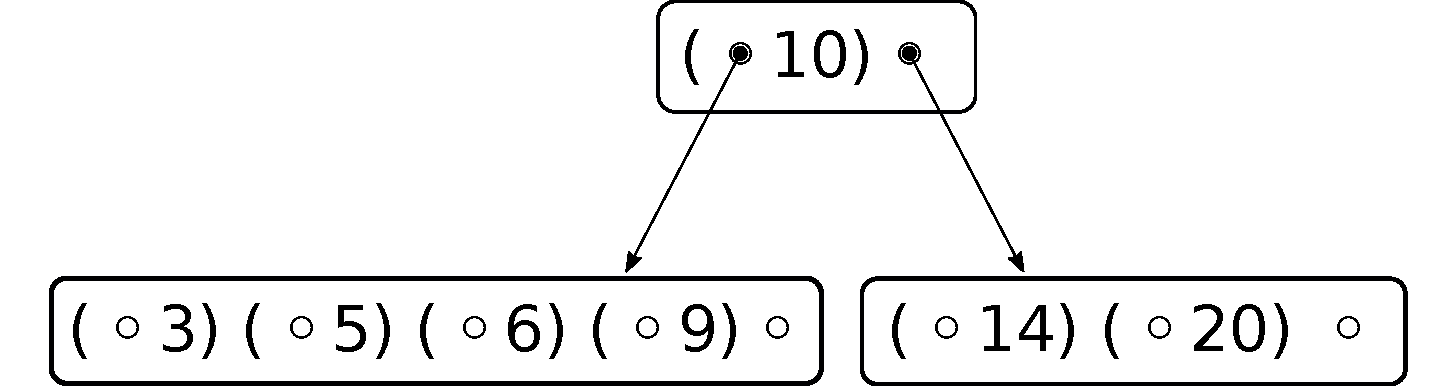
\includegraphics[width=0.48\linewidth]{figures/btree-basic-ins9.pdf}\\
    \vspace*{1cm}
    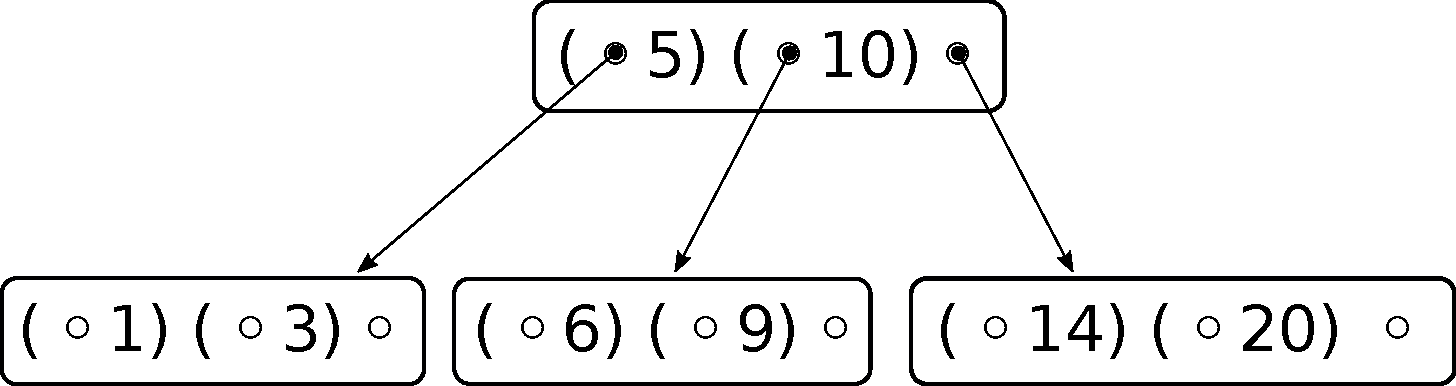
\includegraphics[width=0.48\linewidth]{figures/btree-basic-ins9-ins1.pdf}
    \caption{The tree from \autoref{fig:btree-basic} after 
    successive insertion of $9$ (top) and $1$ (bottom).}
    \label{fig:btree-basic-ins}
\end{figure}
%TODO

To fulfil the Set interface requirements,
we need to show that this function preserves the invariants
and acts the same as inserting element $x$ into the inorder list of the tree.

Note that for the above proofs, a separate notion of height, balancedness and order
was introduced for the $up_i$ datatype.
Height and balancedness are
defined such that the property is invariant to splitting and merging of nodes.
For example, $\height ts\ t = \heightup_i (\node_i k\ ts\ t)$.
Note that this is not the same as applying the original functions
to the tree obtained by tree$_i$.
Order of up$_i$ elements however simply subsumes that all subtrees have
the given order.
Naturally, making a one-element tree of an up$_i$ element will thus
give a node of root-order, while inserting the elements
will not violate the recursive order requirement.

Proving the balancedness invariant requires as additional lemma that
the height is invariant under insertion.
This again follows by induction using the
associativity and commutativity of the maximum function.
Technically, height preservation is only required when modifying balanced
trees, however we have shown the stronger statement that this is even the case for non-balanced trees.
Overall, the fact that the operation does preserve balancedness and height should come at no surprise.
After all, the operations are never directly affecting the height of any tree,
and the two trees generated by splitting a node comprise trees that have been in the tree before as well.

Since the central function to ensure order is the node$_i$ function,
we first show the following lemma:

\begin{lemma}
\label{lem:nodei-order}
    If all children have order $k$ and $\length ts \ge k$ and $\length ts \le 4k+1$
    then all trees in $\node_i k\ ts\ t$ have order $k$.
\end{lemma}

Even though in the case of insertion the length of the list
never exceeds $2k+1$, the statement holds up to $4k+1$.
The statement is proven by case distinction whether $\length ts \le 2k$.
Looking at the definition in \autoref{lst:ins-fun}
we see that if this is the case nothing happens and the lemma is trivial.
In case $\length ts > 2k$, a split occurs.
The median element is passed up as a seperator, leaving
$\lfloor\frac{\length ts}{2}\rfloor$ and $\lceil\frac{\length ts}{2}\rceil - 1$
elements for the left and right node respectively.
Given the constraint on the maximum length of $ts$
this will always be below or equal $2k$.
Further, as we require a size of at least $2k+1$ elements for a split to occur,
the resulting nodes each have at least $k$ elements.
The argument hardly changes comparing the two upper bounds,
but this fact can now be used for merging nodes in the deletion function as well.
With this, the order invariant follows quite directly by induction.

Since the invariant on B-Trees only requires $\order^r k$ on the
root, we additionally derive versions of the invariants
for root order.
They are straightforward however as all trees in the inductive case
have $\order k$, for which preservation was already proven.
Putting things together, we obtain preservation of the invariants

\begin{theorem}
    $\order^r_k t \wedge \bal t \Longrightarrow
    \order^r_k (\insertfun_k x\ t) \wedge \bal (\insertfun_k x t)$
\end{theorem}

The set interface further requires the following fact.
\begin{theorem}
    \label{thm:ins-set}
    $\order_k t \wedge \bal t \wedge \sorted  (\inorder t)\Longrightarrow
    \inorder (\insertfun_k x\ t) = \insertfun_{list} x\ (\inorder t)$
\end{theorem}

Looking at the ins function in \autoref{lst:ins-fun},
we see that in an inductive proof the main obligation
is to argue for the choice of the subtree in case of recursion.
Similar to the proof of \autoref{thm:isin-set},
we use two auxiliary lemmas, that turn the remaining
proof in simple case distinctions and chains of equations.

\begin{lemma}
    $\sorted(\inorder (Node\ ts\ t)) \wedge \splitfun ts\ x = (ls, rs) \Longrightarrow$ \\
    $\inslist (\inorder (Node\ ts\ t))) = \inorder ls @ \inslist x (\inorder rs @ \inorder t)$
\end{lemma}

\begin{lemma}
    $\sorted (\inorder (Node\ ts\ t)) \wedge \splitfun ts\ x = (ls, (sub,sep)\#rs) \wedge sep \neq x \Longrightarrow$ \\
    $\inslist (\inorder ((sub,sep)\#rs) @ \inorder t)) = \inslist x\ (\inorder sub) @ sep \# \inorder rs @ \inorder t$
\end{lemma}

The only case not covered by the above lemmas is the case $sep = x$.
In that case, the tree does not change.
This is due to the fact that $x$ is already in the set represented by the tree
and hence does not need to be inserted.
The same happens when inserting $x$ into a list that already contains $x$
(i.e. the inorder of the tree),
which follows simply by induction on the list.

\begin{lemma}
    $\sorted xs \wedge x \in \setfun xs \Longrightarrow \inslist x\ xs = xs$
\end{lemma}


\subsection{Deletion}

% TODO delete
% TODO move abstract discussion to introduction
%-------------------------------------------------
Generally, elements are removed from the leaves only.
If the element to be deleted resides in an inner node,
it is replaced by the maximal lesser or minimal greater
element in the tree, which always resides in a leaf.

After deletion, the nodes may need rebalancing in order
to ensure the order property.
A node having less than $k$ elements is called to have "underflow".
However, opposing to the insertion function,
the exact procedure to handle underflow varies strongly in the literature.
In most of the popular modern references, %TODO citations
the primary remedy to underflow is a "steal"
from the left or right sibling.\parencite{DBLP:books/daglib/0023376}
If the left or right sibling has more than $k$ elements,
one of the neighboring elements may be moved out for increasing
the size of the current node.
Only in case that both siblings have left only $k$ elements,
a kind of reversal of the insertion split is conducted:
One of the siblings and the node itself are merged to form
a new, bigger node of valid order.

Following the description of \parencite{DBLP:journals/acta/BayerM72},
as done by \parencite{Fielding80},
the two cases can be treated identically.
If a node has less than $k$ elements,
merge it with one of its siblings.
% TODO note that someone(tm) said this is more efficient then stealing
If the resulting node has more than $2k$ separators,
it will be split in half again, just as if an overflow occurred.
According to \dots this may even be more efficient than stealing single values.
First of, the resulting node is less likely to underflow again.
If it had stealt only one item, it would certainly underflow at the next
deletion.
Further, the node to merge with has to be read from memory anyways.
The cost of moving around the memory
is hence negligible compared to the cost of another underflow.

%-------------------------------------------------

\begin{figure}
\begin{lstlisting}[mathescape=true, language=Isabelle,label={lst:rebalance-def},
    caption={The rebalancing functions}]
fun rebalance_middle_tree where
  rebalance_middle_tree k ls Leaf sep rs Leaf = (Node (ls@(Leaf,sep)#rs) Leaf) |
  rebalance_middle_tree k ls (Node mts mt) sep rs (Node tts tt) = (
    if length mts $\ge$ k $\wedge$ length tts $\ge$ k then
        Node (ls@(Node mts mt,sep)#rs) (Node tts tt)
    else (
        case rs of [] $\Rightarrow$ (
            case node$_i$ k (mts@(mt,sep)#tts) tt of
                T$_i$ u $\Rightarrow$ Node ls u |
                Up$_i$ l a r $\Rightarrow$ Node (ls@[(l,a)]) r
            ) |
        (Node rts rt,rsep)#rs $\Rightarrow$ (
            case node$_i$ k (mts@(mt,sep)#rts) rt of
                T$_i$ u $\Rightarrow$ Node (ls@(u,rsep)#rs) (Node tts tt) |
                Up$_i$ l a r $\Rightarrow$ Node (ls@(l,a)#(r,rsep)#rs) (Node tts tt)
            )
        )
    )

fun rebalance_last_tree where
    rebalance_last_tree k ts t = (
        case last ts of (sub,sep) $\Rightarrow$ rebalance_middle_tree k (butlast ts) sub sep [] t
    )
\end{lstlisting}
\end{figure}

The described procedures are implemented here with a
certain flavor due to the setup of B-Trees.
The "rebalancing" as implemented in \autoref{lst:rebalance-def}
comprises merging and splitting neighboring nodes.
For simplicity of the function and proofs, we always
merge with the right sibling.
The only exception, which is unavoidable due to the asymmetry of the data structure,
is an underflow in the last tree.
It will be merged with the second-to-last tree.

The other detail is regarding the split\_max function
defined in \autoref{lst:del-def}.
Since the last tree of the node is explicitly stored in each Node
and the left subtree of a separator lies within the same
pair inside the node list, it is significantly
easier to obtain the maximum of the left subtree
than the minimum of the right subtree.
Therefore we will always swap inner separators with the former element.
%---------------------------------------------------------

The most interesting property for the rebalancing operations is the order property,
which is meant to be restored after potential underflows.
It is important to note here that we cannot guarantee
that at least one element remains in the node.
However we can guarantee that all subtrees of the result are of order $k$
and that there are no more than $2k$ elements in the result.
This state is denoted as $\order^a_k$.

\begin{lemma}
    If all subtrees are of order k except for sub or t, of which one may have order$^a$ k,
    and all subtrees have equal height $\Longrightarrow$
    $\order^a_k (\rebalancemt_k ls\ sub\ sep\ sep\ rs\ t)$
\end{lemma}

For this proof, we re-use \autoref{lem:nodei-order},
as two nodes of order $k$ will always contain
a maximum of $4k+1$ separators.
The case that the subtree and separator list becomes zero
is exactly when a root with minimal size underflows.
After this operation the tree shrinks in height.
The shrinked tree then is exactly the one remaining subtree in the original node.
See the operation $reduce\_node$ in \autoref{lst:del-def} for the exact implementation
of this step.

\begin{figure}
\begin{lstlisting}[mathescape=true, language=Isabelle,label={lst:del-def},
    caption={The $delete$ function}]

fun split_max where
    split_max k (Node ts t) = (
        case t of Leaf $\Rightarrow$ (
            let (sub,sep) = last ts in (Node (butlast ts) sub, sep)
        ) |
        _ $\Rightarrow$ case split_max k t of (sub, sep) $\Rightarrow$
                (rebalance_last_tree k ts sub, sep)
        )

fun del where
    del k x Leaf = Leaf |
    del k x (Node ts t) = (
    case split ts x of (ls,[]) $\Rightarrow$
        rebalance_last_tree k ls (del k x t) |
    (ls,(sub,sep)#rs) $\Rightarrow$
        if sep $\neq$ x then
            rebalance_middle_tree k ls (del k x sub) sep rs t
        else if sub = Leaf then
            Node (ls@rs) t
        else let (sub_s, max_s) = split_max k sub in
            rebalance_middle_tree k ls sub_s max_s rs t
    )
 
fun reduce_root where
    reduce_root Leaf = Leaf |
    reduce_root (Node ts t) = (case ts of
        [] $\Rightarrow$ t |
        _ $\Rightarrow$ (Node ts t)
    )
 
fun delete where delete k x t = reduce_root (del k x t)
\end{lstlisting}
\end{figure}

\begin{figure}
    \centering
    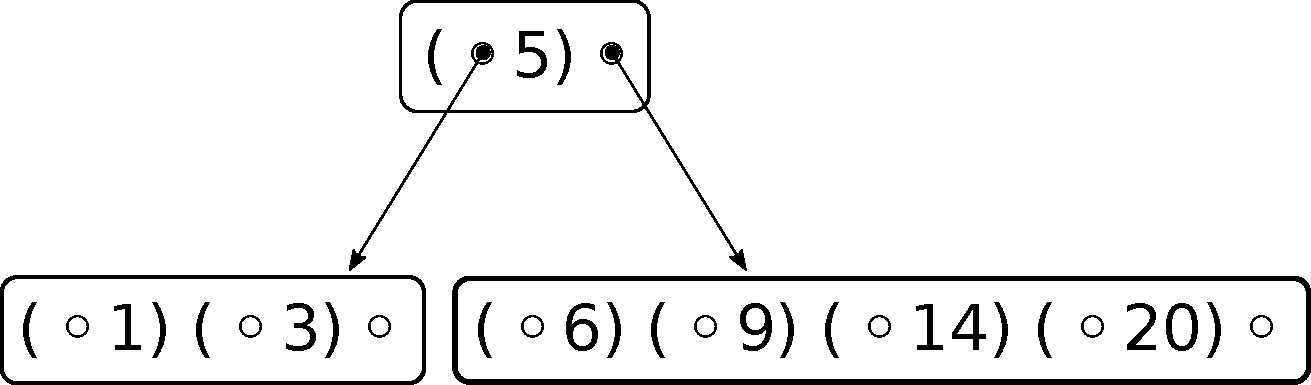
\includegraphics[width=0.48\linewidth]{figures/btree-basic-ins9-ins1-del10.pdf}\\
    \vspace*{1cm}
    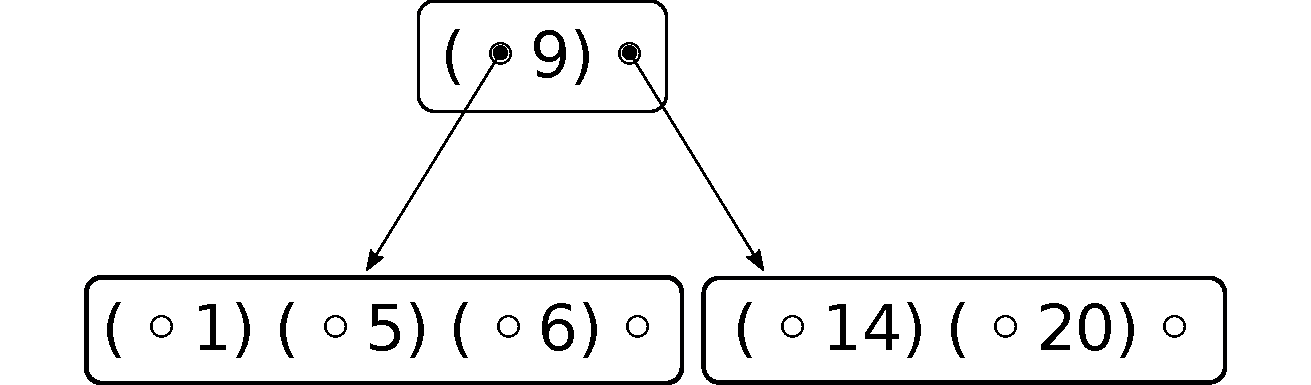
\includegraphics[width=0.48\linewidth]{figures/btree-basic-ins9-ins1-del10-del3.pdf}
    \caption{The tree from \autoref{fig:btree-basic-ins} after 
    successive deletion of $10$ (top) and $3$ (bottom).
    Note how the final result differs from approaches that would only steal single elements
    from neighbors to hanlde underflow.}
    \label{fig:btree-basic-del}
\end{figure}

From this fact follows further, that for the results of all intermediate functions
in the deletion process, $\order^a k$ of the results can be guaranteed.
Since the last subtree in the result of deletion has $\order k$,
and for more than one subtree the node has root order,
the result of $\deletefun$ always has at least $\order^r k$.

The balancedness invariance follows similarly to
insertion by first showing height invariance % TODO reference
using the associativity and commutativity of the maximum operation.
Its proofs are interleaved with the other proofs,
since the intermediate functions, especially
split\_max and $\rebalancemt$, are only well defined for balanced trees
and split\_max requires at least one element in the node list, an equivalent
to $\order^r k$.

% TODO this might be conclusion
The actual proofs in this work have been written to use only
minimal requirements on the input.
For example in \autoref{lem:splitmax-inorder}, rather than
requiring balancedness and $\order k$ for $k > 0$ on the full tree,
it is only required that the node has at least two children
and the last two have equal height and that the last tree has the same, recursive property.
Using the latter property was beneficial during the proof,
as the less restrictive requirements simplify satisfying
the preconditions for applying the induction hypothesis.
However this also called for more lemmas that show that
the weaker property is satisfied in valid B-Trees.
Nevertheless, generating the most general lemmas usually turned out to be
very useful, for example in \autoref{lem:nodei-order}, yielding the reusability of $\node_i$ for
merging two nodes in deletion.
Another use case was the applicability of weaker properties
even when temporary violations
of the general invariant were observed during deletion,
such as in the $del$ function in \autoref{lst:del-def}.
%---------------------------------

Putting together the proofs on balancedness and
order, we obtain the important fact about the invariant preservation of the deletion function.
Note that we now require $k > 0$.
The reason is that, while it was not too important for most of the proofs until now,
B-Trees do only work for positive $k$.
If $k = 0$, rebalancing would not always work anymore
as we could not be certain to have at least two subtrees per node.

\begin{theorem}
    $k > 0 \wedge \order^r_k t \wedge \bal t \Longrightarrow
    \order^r_k (\deletefun_k x\ t) \wedge \bal (\deletefun_k x t)$
\end{theorem}

In order to prove that $delete$ acts the same as
$delete_{list}$ on the inorder of the tree,
we need to show some inorder properties for the intermediate functions.
For the $del$ helper function, 
we use the same specialized lemams
as for \autoref{thm:isin-set} and \autoref{thm:ins-set}
and induct over the execution of the del-function.
% TODO state or no state?

Rather than stating the specialized lemmas again at this point, we would like to point
out the elegance of the inorder method at this point.

The reason the rebalancing functions preserve the sortedness and set properties
is plain when considering the inorder view of the tree:
it does not change at all.
A manual proof about the set and sortedness properties
would require complicated, unnecessarily lengthy proofs.
For the inorder view, 
since the results can be easily simplified, even without recursive calls,
the property follows automatically.

\begin{lemma}
    \label{lem:rebalance-inorder}
    All subtrees have the same height $\Longrightarrow$ \\
    $\inorder (\rebalancemt_k ls\ sub\ sep\ rs\ t) = \inorder (Node (ls@(sub,sep)\#rs)\ t)$
\end{lemma}

Considering the function split\_max,
the standard approach would require showing
tideously that the element returned is in fact the maximum of the whole tree
and showing that the remaining tree union the maximum element
gives the whole original tree set.
Instead we simply show the following,
comprising both facts:

\begin{lemma}
    \label{lem:splitmax-inorder}
    If t has more than two subtrees, and the last two are equally high, then
    $\inorder (\splitmax_k t) = \inorder t$
\end{lemma}

This fact follows easily by induction on the computation of split\_max,
using \autoref{lem:rebalance-inorder}.

The reason that the proof of these functions follows so easily
lies in the intention behind the definition of both functions.
Together with the fact that the remaining tree is balanced and
fulfils a certain order property, the inorder view
is not meant to change.
We obtain the same elements, in the same order,
just now in a configuration from which we can obtain
a new, valid, B-Tree.

Finally we obtain the last important property of the set interface.
\begin{theorem}
    $k > 0 \wedge \order^r_k t \wedge \bal t \wedge \sorted  (\inorder t)\Longrightarrow
    \inorder (\deletefun_k x\ t) = \deletefun_{list} x\ (\inorder t)$
\end{theorem}

With this, the implementation the set interface by
our implementation of B-Trees is proven correct.
The next step towards imperative B-Trees is to implement
an imperative refinement of the set operations.

\chapter{Imperative B-Trees in Isabelle}\label{chapter:imp-set}

In the previous chapter, we have seen
an abstract definition of B-Trees and the reasoning
behind its correct implementation of the set interface.
However, the specification would not yield 
efficiently executable code.
% main difference: specify allocation of data
The reason is that the abstract specification works with
the ephemeral datatypes of nodes and lists.
This way, trivially no data is unknowingly
modified or corrupted,
however this is at the cost of computational efficiency.
In order to obtain an efficient implementation
on mutable objects,
we specify imperative code and show that
it refines the abstract specification.

\section{Refinement to Imperative/HOL}

The proofs of correct behavior for our imperative
code are stated with separation logic in Isabelle/HOL.
The framework for this was provided by
\parencite{DBLP:journals/jar/Lammich19}.
It provides a way to reason about mutable resources
that lie in separated parts of an external heap,
an abstracted memory device.
The assumptions on the state of the heap are called \textit{assertions}.
They are specified as formulae that hold for specific heap states.
Assertions that are required to understand
this work follow.

\begin{itemize}
    \item \textit{emp} holds for the empty heap
    \item \textit{true} and \textit{false} hold for every and no heap respectively
    \item $\uparrow(P)$ holds if the heap is empty and predicate $P$ holds
    \item $a \mapsto_a as$ holds if the heap at position $a$ is reserved and contains
    an array representing $as$.
    \item $a \mapsto_r x$ holds if the heap at position $a$ is reserved and contains
    value $x$ where $x$ is of some type $'a::heap$
    \item $\exists_A x. P x$ holds if there exists some $x$ such that predicate P
    holds on the heap for given $x$.
    \item $P_1 * P_2$ holds if each assertion holds on its part of the heap
    and the areas of the heap described by each assertion are non-overlapping
\end{itemize}

In general, refinement relates a concrete data structure
to an abstract structure via some refinement assertion.
An example for such a refinement assertion are the id assertion and the
list assertion, relating lists given a refinement
assertion between the elements of the first and second list.

\begin{lstlisting}[mathescape=true, language=Isabelle]
definition id_assn a b = $\uparrow$(a = b)

fun list_assn :: ('a $\Rightarrow$ 'c $\Rightarrow$ assn) $\Rightarrow$ 'a list $\Rightarrow$ 'c list $\Rightarrow$ assn where
  list_assn P [] [] = emp
| list_assn P (a#as) (c#cs) = P a c * list_assn P as cs
| list_assn _ _ _ = false
\end{lstlisting}

We can then specify Hoare Triples on assertions.

\begin{definition}
    $\langle$ P $\rangle$ c $\langle \lambda r. $ Q r $\rangle$ \\
    holds iff if assertion $P$ holds on some heap before operation $c$
    is executed on the heap,
    and operation $c$ returns some $r$, then assertion $Q$ holds
    on the modified heap for $r$.
\end{definition}

A simple example Hoare Triple is 
$\langle$ id\_assn $a$ $b$ $\rangle$ return $b$ $\langle \lambda r.$ id\_assn $a$ $r$ $\rangle$.
In the refinement process, we will use more complex relationship assertions
on the input $b$ to some object $ab$ and show that the value $r$ returned
by the imperative program satisfies a relationship to the output of the refined
function applied to $ab$.
Further we use the shorthand notation $\langle\ P\ \rangle\ c\ \langle \lambda r.\ Q\ r\ \rangle_t$
which stands for $\langle\ P\ \rangle\ c\ \langle \lambda r.\ Q\ r\ * true\ \rangle$.
Since $true$ holds for any heap, this part of the statement may be used to subsume
all temporary and discarded variables.

Refining all set operations from \autoref{chapter:abs-set}
yields imperative code
that stores data on the heap
and operates with more efficient destructive updates.
We do not need to show that the operations themselves
satisfy the requirements of the set interface.
Instead we merely need to show that the imperative code
acts on a concretized version of the B-Trees
the same way as the abstract operations on the abstract version.

% TODO note what to introduce here
% abstract idea: implementation that has same effect on concrete ds
% as abstract function on abstract ds
% TODO short intro hoare triples and notation here
% *  and \uparrow

\subsection{Refinement of abstract lists}

In the imperative collection framework\parencite{DBLP:journals/jar/Lammich19},
the abstract datatype list is usually
refined to a dynamic array like data structure.
It comprises an array and a natural number,
where the latter denotes the current number of elements
stored in the array.
B-Tree nodes do not always contain a constant number of elements,
which is why this property should be transferred to
the data structure refining key-value lists. 

% TODO intended physical storing of B-Tree on pages of memory
% --> partially filled array, non-dynamic!
However, dynamic arrays are designed to grow and shrink
as elements are inserted.
B-Trees were invented to be stored on slow hard disks.
As one disk access loads a chunk of data into a page of main memory,
nodes of this size would make the most efficient use of the loading times. \parencite{DBLP:journals/acta/BayerM72}
%TODO give clear reason
Therefore the data structure to store the node content
should reserve a fixed amount of data, independent
of the actual number of keys and children.

Based on the definition of dynamic arrays in the 
imperative collection framework,
we therefore introduce a simple data structure
that keeps count of currently inserted elements,
but does neither grow nor shrink.
Abstractly, we refine lists in the functional B-Trees to this
data-structure.
A list $l$ is represented by a partially filled array $(a,n)$,
if the array $a$ represents a list $l'$, of which the first $n$
elements form list $l$.
Formally,

\begin{lstlisting}[mathescape=true, language=Isabelle]

typedef 'a pfarray = 'a array $\times$ nat

definition is_pfa where c l $\equiv$
    $\lambda$(a,n). $\exists_A$ l'. a $\mapsto_a$ l' *  $\uparrow$(c = length l' $\wedge$ n $\le$ c $\wedge$ l = (take n l'))
\end{lstlisting}

where $c$ is the $capacity$ of the array, that is the actual allocated size
of the array on the heap.
From the abstract specification alone
it is not clear which operations are supposed to be conducted
in-place and which will require copying data.
To obtain the most efficient code we therefore manually
define the following operations to replace complex composite
operations based on list construction and concatenation.

% abstract function has length, insertion, take/drop
% --> concrete implementations
\begin{figure}
\begin{lstlisting}[mathescape=true, language=Isabelle,label={lst:pfarray-def},
    caption={Important Partially Filled Array functions for Insertion.}]
definition pfa_length $\equiv$ $\lambda$(a,n). return n

definition pfa_get $\equiv$ $\lambda$(a,n) i. Array.nth a i

definition pfa_set $\equiv$ $\lambda$(a,n) i x. do {
    a $\leftarrow$ Array.upd i x a;
    return (a,n)
}

definition pfa_shrink k $\equiv$ $\lambda$(a,n). return (a,k)

definition pfa_shrink_cap  k $\equiv$ $\lambda$(a,n). do {
    a' $\leftarrow$ array_shrink a k; (* returns an array with the given actual size, potentially reallocated*)
    return (a',min k n)
}

definition pfa_drop $\equiv$ $\lambda$(src,sn) si (dst,dn). do {
    blit src si dst 0 (sn-si);
    return (dst,(sn-si))
}

definition pfa_insert $\equiv$ $\lambda$(a,n) i x. do {
  a' $\leftarrow$ array_shr a i 1; (* shifts elements to the right by 1 *)
  a'' $\leftarrow$ Array.upd i x a;
  return (a'',n+1)
}

definition pfa_ensure $\equiv$ $\lambda$(a,n) k. do {
  a' $\leftarrow$ array_ensure a k default; (* returns an array with given minimal size, potentially reallocated *)
  return (a',n)
}

definition pfa_insert_grow  $\equiv$ $\lambda$(a,n) i x. do {
  a' $\leftarrow$ pfa_ensure (a,n) (n+1);
  a'' $\leftarrow$ pfa_insert a' i x;
  return a''
}

$\dots$
\end{lstlisting}
\end{figure}

% TODO also include what the rule gives us?

During the splitting of nodes, a part of the overflowing
list is copied into another array.
The operation to copy data is based on the function $blit$,
that copies a slice of an array to the starting position of another array.
The function already existed in the standard collection and could be reused
to define the $pfa\_drop$ function in \autoref{lst:pfarray-def}, which in this implementation copies data to a new array.

The $blit$ function is however not capable of correctly copying data
within the array, as required for efficient in-place insertion and deletion.
A suitable function, called $sblit$, was hence added in the course of this project.
The relevant addition is to differentiate between copying elements
from higher to lower indices or from lower to higher indices.
Depending on the direction of the copy, it is relevant
in which order to copy singleton elements so that in case
of overlapping ranges no elements are overwritten before being copied.
By adding a function that copies elements in reverse order
and conditionally calling either copy function,
loss-free in-place copying was achieved.
The resulting function is conveniently agnostic to the direction
of the copying, just as the respective implementations
in target languages.\footnote{
    See for example \href{https://caml.inria.fr/pub/docs/manual-ocaml/libref/Array.html}{the specification of \texttt{Array.blit} in Ocaml} or
    the \href{https://smlfamily.github.io/Basis/array-slice.html\#SIG:ARRAY_SLICE.copy:VAL}{\texttt{ArraySlice.copy} specification in SML}.
}
The $pfa\_insert$ function in \autoref{lst:pfarray-def} makes
implicit use of in-place copying by calling a function to shift elements
to the right by one.
The element to be inserted is then placed in the remaining free spot.

For all functions in \autoref{lst:pfarray-def},
appropriate Hoare-Triples were derived.
All triples are straightforward to derive which is why they are not
listed listed in great detail.
To roughly sketch the obtained lemmas, the two examples
\texttt{pfa\_drop} and \texttt{pfa\_shrink} are investigated below.
The most important difference is whether
the operations are destructive (in-place) or not.
For most operations, the approach that required the least
memory allocations was chosen.\footnote{
    The only exception is node$_i$, which in the case of overflow
    currently requires temporary allocation of an array that holds more than $2k$ elements.
}

\begin{lemma}
    $k \le \length s \wedge (\length s - k) \le dn \Longrightarrow$ \\
    \begin{center}
    $\langle \pfarraycap$ sn s si * $\pfarraycap$ dn d di $\rangle$ \\
    $\pfadrop$ si k di \\
    $\langle\lambda di'. \pfarraycap$ sn s si * $\pfarraycap$ dn ($\drop$ k s) di' $\rangle$
    \end{center}
\end{lemma}

The array $si$ stays untouched.
This fact is expressed by the fact that the term about its relationship to $s$
is still available in the postcondition of the triple.
The only thing that changed is the content of $di$.\footnote{
    In the actual proof, where possible, we even show that the array itself has not changed
    (i.e. has not been reallocated).
    The correct notation does however not yield high readability
    and is hence abstracted here.
}
The $take$ function was refined differently.
The cheapest and in our context consistent option is
reducing the number of elements that are considered part of the represented list
from $n$ to $k$.
The result is that the original array gets modified and we loose any information
about the content that is written beyond given $k$.

\begin{lemma}
    $k \le \length s\Longrightarrow$ \\
    \begin{center}
    $\langle \pfarraycap$ sn s si$\rangle$
    $\pfashrink$ si k
    $\langle\lambda si'. \pfarraycap$ sn ($\take$ k s) si' $\rangle$
    \end{center}
\end{lemma}

With these operations and suitable Hoare-Triples about them,
we have all the tools required to refine the abstract set implementation.
The only missing piece is an imperative split function.
% TODO more about sblit?

\section{Set-Operations}

With refinements for all basic components in the B-Tree set operations,
the B-Tree datatype itself can be refined.
Rather than actually storing nodes within lists,
the B-Tree nodes are supposed to be stored in the heap,
only storing pointers to other nodes in the element list.
Since the Imperative Refinement Framework does not support null pointers,
we store heap reference options instead.
Thus None represents leafs or empty trees.
The physical B-Tree datatype does hence only need to cover the case
of actually being an inner node.

\begin{lstlisting}[mathescape=true, language=Isabelle]
datatype 'a btnode =
    Btnode ('a btnode ref option*'a) pfarray 'a btnode ref option
\end{lstlisting}

Note the similarity to \autoref{lst:btree-def},
only that "btree" was replaced by "btnode ref option"
and "list" was replaced by "pfarray".

An abstract B-Tree is represented by such a physical node
if all references on subtrees represent the corresponding
abstract subtrees and all keys are the same.

\begin{lstlisting}[mathescape=true, language=Isabelle]
fun btree_assn :: nat $\Rightarrow$ 'a::heap btree $\Rightarrow$ 'a btnode ref option $\Rightarrow$ assn where
  btree_assn k Leaf None = emp |
  btree_assn k (Node ts t) (Some a) = 
 ($\exists_A$ tsi ti tsi'.
      a $\mapsto_r$ Btnode tsi ti
    * btree_assn k t ti
    * is_pfa (2*k) tsi' tsi
    * list_assn ((btree_assn k) $\times_a$ id_assn) ts tsi'
    ) |
  btree_assn _ _ _ = false

abbreviation blist_assn k $\equiv$ list_assn ((btree_assn k) $\times_a$ id_assn)

\end{lstlisting}

It seems a little bit awkward that the definition
includes two relationships regarding only the list of elements in the subtree.
The reason is that there are two steps of refinements going on.
First all elements in a list are refined to their physical counterpart.
This fact is expressed by the list assumption term in the assumption.
Second, the list itself is refined to an array.
This is expressed in the term about the partially filled array relationship.
Since the list assumption makes recursive use of the
B-Tree assumption, this is however a very convenient
way of expressing the desired relationship.

Using the parameters of \texttt{is\_pfa},
note that we can specify that every node of a B-Tree should have
capacity for $2k$ elements.

\subsection{The split function}
\label{sec:imp-split}

To implement any set operations we again need a split operation.
However, what split function exactly will be used can be abstracted again.
The only important thing is that it refines an abstract split function.
Imperative split functions should be efficient and as such not actually
split an array in half and return it the way the abstract function did.
Rather than that the function should return the index of the subtree
in which should be recursed.
The refinement condition derived from this relationship is as follows.

\begin{lstlisting}[mathescape=true, language=Isabelle]
definition split_relation xs $\equiv$ $\lambda$(ls,rs) i. i $\le$ length xs $\wedge$ ls = take i xs $\wedge$ rs = drop i xs
\end{lstlisting}

A very useful alternative statement of the relationship follows automatically.

\begin{lemma}
    $\splitrelation xs\ (ls,rs)\ i = (xs = ls@rs \wedge i = \length ls)$
\end{lemma}

From this, we characterize the desired imperative
split function \texttt{imp\_split} by its Hoare-Triple.

\begin{align*}
    \langle & \pfarraycap c\ tsi\ a * \blistassn k\ ts\ tsi *  true \rangle \\
            & \impsplit a \\
\langle\lambda i. & \pfarraycap c\ tsi\ a * \blistassn k\ ts\ tsi * \uparrow(\splitrelation ts\ (\splitfun ts p)\ i)\rangle_t
\end{align*}

Just as with the abstract implementation,
the imperative refinements can be built with this characterization alone.
However this time we are actually interested in finding an
efficient split and will spend some time finding
a good split function.
%TODO move to after the set operations?

In the imperative context, we prefer not to directly
implement the recursive function from \autoref{fig:linear_split}
but we embark on the exercise of using a while loop.
The implementation in \autoref{lst:imp-linear-split}
is very basic but good for getting to know
the usage of while loops in imperative HOL.
Every iteration, an index on the array is moved forward by one.
The main part is done in the loop head - if we
are within the array bounds,
we obtain the current separator and check if it is
smaller than the partitioning element.
We return the first index, at which the separator is greater or equal.

\begin{figure}
\begin{lstlisting}[mathescape=true, language=Isabelle, caption={The imperative linear split},
    label={lst:imp-linear-split}]
definition lin_split :: ('a::heap $\times$ 'b::{heap,linorder}) pfarray $\Rightarrow$ 'b $\Rightarrow$ nat Heap where
    lin_split $\equiv$ $\lambda$ (a,n) p. do { 
   
        i $\leftarrow$ while  
            ($\lambda$i. if i<n then do { 
            (_,s) $\leftarrow$ Array.nth a i; 
            return (s<p) 
            } else return False)  
            ($\lambda$i. return (i+1))  
            0; 
                
        return i 
    }
\end{lstlisting}
\end{figure}

This function behaves quite different to the abstract linear split
that was implemented before.
Therefore, proving that it refines the abstract function requires a small detour.
We first express and show the most basic, non-trivial result of the function.
With the help of that we may then show that the result is the same as the result
of applying the abstract function.

We begin with stating a simple matching Hoare Triple
for the function.
It follows by supplying the loop invariant,
which is that all elements up to the current $i$
are smaller than the partitioning element.
Further the invariant contains the fact that the array stays unchanged.
% TODO state loop invariant explicitely

\begin{lemma}
    \begin{align*}
        \langle &\pfarraycap c\ xs\ (a,n)\rangle \\
                  &\linsplit\ (a,n)\ p \\
        \langle \lambda i. & \pfarraycap c\ xs\ (a,n) \\
        * &\uparrow(i \leq n 
            \wedge (\forall j < i. snd (xs!j) < p) 
            \wedge (i<n \longrightarrow snd (xs!i) \geq p)) \rangle_t 
    \end{align*}
\end{lemma}

For unexciting reasons, this post condition
actually suffices to imply that there exists a split relation
to the result of an abstract split function.
Specifically, we use the abstract split function from
\autoref{fig:linear_split}. %TODO or explain why a different function was used
This is great to know since the previous lemma
follows directly from the computation and is closely related
to the loop invariant.\footnote{
    Another reason for excitement is that now we can specify an imperative B-Tree
    specification without any reference to the abstraction.
    We simply always use the well known split function in the abstraction
    and only require a post condition similar to the one just shown
    on the imperative split function.
}
With this assurance we approach the binary split.

The binary split in \autoref{lst:imp-binary-split} conducts a binary search on
the list of elements.
Rather than walking through the array,
it narrows down a windows on the array that becomes smaller with
every iteration.
In the final iteration,
the windows must have narrowed down to a single element,
which is the result.

\begin{figure}
\begin{lstlisting}[mathescape=true, language=Isabelle, caption={The imperative binary split},
    label={lst:imp-binary-split}]
    definition bin_split :: ('a::heap $\times$ 'b::{heap,linorder}) pfarray $\Rightarrow$ 'b $\Rightarrow$ nat Heap 
    where 
      bin_split $\equiv$ $\lambda$(a,n) p. do { 
    (low',high') $\leftarrow$ while  
      ($\lambda$(low,high). return (low < high))  
      ($\lambda$(low,high). let mid = ((low  + high) div 2) in 
       do { 
        (_,s) $\leftarrow$ Array.nth a mid; 
        if p < s then 
           return (low, mid) 
        else if p > s then 
           return (mid+1, high) 
        else return (mid,mid) 
       })  
      (0::nat,n); 
    return low' 
  }
\end{lstlisting}
\end{figure}

A detailed analysis of binary search algorithms
may be found in \parencite{DBLP:journals/csedu/Montague91},
which has served as an orientation for the derived algorithm.
Since the introduction of products as list elements
adds another layer of complexity for the simplifier.
Therefore a binary split algorithm on lists that contain
only single elements has been derived first.
Surprisingly, obtaining the same Hoare Triple
as for the linear split requires merely
a slightly more complex loop invariant
invocation of a number of algebraic lemmas.
% TODO note/explain loop invariant?
The additional requirement here is naturally
that the list of separators must be sorted.

\begin{lemma} $\sorted (\separators xs) \Longrightarrow$ \\
    \begin{align*}
        \langle &\pfarraycap c\ xs\ (a,n)\rangle \\
                  &\binsplit\ (a,n)\ p \\
        \langle \lambda i. & \pfarraycap c\ xs\ (a,n)
        * \uparrow(i \leq n 
            \wedge (\forall j < i. snd (xs!j) < p) 
            \wedge (i<n \longrightarrow snd (xs!i) \geq p)) \rangle_t 
    \end{align*}
\end{lemma}

Since we know that this implies equivalence to the abstract split function
and sortedness of the separators is guaranteed by the sortedness
invariant of the B-Trees,
we can safely use this function for specifying
the set operations.

%TODO Note the choice of a while-loop for efficiency
%TODO The split function can be implemented linearly (easier, proof of concept)
% but due to abstraction of functionality may use binary split as well.

\subsection{The isin function}

The imperative set operations do quite directly follow
from the refinement the abstract operations.
Pointers need to be dereferenced, modified and updated.
Functions such as length need to be called and have their result
stored explicitly before use.
Other than that, the definition of the imperative isin in \autoref{lst:imp-isin-fun}
function should bare no surprises.
Note that it makes use of the function \texttt{imp\_split}
which is an arbitrary split function that has the Hoare Triple
specified in \autoref{sec:imp-split}.

\begin{figure}
\begin{lstlisting}[mathescape=true, language=Isabelle, label={lst:imp-isin-fun},
    caption={The imperative isin function}]
partial_function (heap) isin :: 'a btnode ref option $\Rightarrow$ 'a $\Rightarrow$  bool Heap
  where
    isin p x =
  (case p of
     None $\Rightarrow$ return False |
     (Some a) $\Rightarrow$ do {
       node $\leftarrow$ !a;
       i $\leftarrow$ imp_split (kvs node) x;
       tsl $\leftarrow$ pfa_length (kvs node);
       if i < tsl then do {
         s $\leftarrow$ pfa_get (kvs node) i;
         let (sub,sep) = s in
         if x = sep then
           return True
         else
           isin sub x
       } else
           isin (last node) x
    }
)
\end{lstlisting}
\end{figure}

The Hoare Triple to argue that this is a refinement of the abstract operation
is as follows (where $abs\_split$ refers to some abstract implementation
of the set operations from \autoref{chapter:abs-set}):

\begin{lemma} $\sorted (\inorder t) \Longrightarrow$ \\
\begin{align*}
   \langle &\btreeassn k\ t\ ti\rangle \\
           &\isinfun ti\ x \\
   \langle \lambda r. &\btreeassn k\ t\ ti * \uparrow(\isinfun t\ x = r)\rangle_t
\end{align*}
\end{lemma}

Note how, in contrast to the abstract specification,
we need to also show that the imperative function does not modify the tree
residing in the heap.
The proof follows by induction on the computation of the abstract isin function.
% TODO conclusion ?
Inside a structured proof skeleton of the induction,
proving the subgoals turned out to be the most
appropriate in an apply style manner.
The only help that the separation automation tool required
is a manually specification of the instantiation for existential quantifiers
for applying the inductive hypothesis. 
% TODO more details?

\subsection{Insertion}

%TODO Description of applying the refinement framework to the insert function
The imperative implementation and derived heap rule of the insertion function follow
the same pattern as the isin function.
The only interesting part is whether and how often new memory is allocated.
An excerpt of the ins function can be seen in \autoref{lst:imp-ins-fun}.
The function includes some optimizations, such as not calling
$\node_i$ if the node is not overflowing.
This is an optimization as otherwise $\node_i$ in
\autoref{lst:imp-nodei-fun} would always allocate a new B-Tree node
rather than updating the current node in place.

To prove that this optimization is valid, the only obligation
is to show that the updated node itself is equivalent
to the node returned by $\node_i$.
Since we are in the branch where the node contains less than $2k$
elements, this is easy to show, providing some intermediate lemmas
that relate concrete node and abstract node in this context.
Adding a lemma on the equivalence between abstract and imperative
$node_i$, we finally obtain a lemma for ins by induction on the computation
of the abstract ins function.

The insertion function incorporates the function $\tree_i$
in much the same way.
Here the proof of equivalence followed automatically.
With the hoare rule for $ins$, we obtain the final desired lemma
on the imperative insertion.

\begin{lemma} $k > 0 \wedge \sorted (\inorder t) \Longrightarrow$ \\
\begin{align*}
   \langle &\btreeassn k\ t\ ti\rangle \\
           &\insertfun k\ x\ ti \\
   \langle \lambda r. &\btreeassn k\ (\insertfun k\ x\ t)\ r\rangle_t
\end{align*}
\end{lemma}

% TODO say something about k?
%Note how we have the additional assumption that $k$ be positive. This was only required to show correct order in the abstract setting.
%Here, the capacity of the root node needs to be specified.
%And since the capacity has to be $2k$ and the node has to hold at least one element


% TODO...
\begin{figure}
\begin{lstlisting}[mathescape=true, language=Isabelle, label={lst:imp-nodei-fun},
    caption={The imperative node$_i$ function}]
definition node$_i$ 
    :: nat $\Rightarrow$ ('a btnode ref option $\times$ 'a) pfarray $\Rightarrow$ 'a btnode ref option $\Rightarrow$ 'a btupi Heap
  where node$_i$ k a ti $\equiv$ do {
      n $\leftarrow$ pfa_length a;
      if n $\le$ 2*k then do {
        a' $\leftarrow$ pfa_shrink_cap (2*k) a;
        l $\leftarrow$ ref (Btnode a' ti);
        return (T$_i$ (Some l))
      }
      else do {
        b $\leftarrow$ (pfa_empty (2*k)
            :: ('a btnode ref option $\times$ 'a) pfarray Heap);
        i $\leftarrow$ split_half a;
        m $\leftarrow$ pfa_get a i;
        b' $\leftarrow$ pfa_drop a (i+1) b;
        a' $\leftarrow$ pfa_shrink i a; 
        a'' $\leftarrow$ pfa_shrink_cap (2*k) a';
        let (sub,sep) = m in do {
          l $\leftarrow$ ref (Btnode a'' sub);
          r $\leftarrow$ ref (Btnode b' ti);
          return (Up$_i$ (Some l) sep (Some r))
        }
      }
    }

\end{lstlisting}
\end{figure}

\begin{figure}
\begin{lstlisting}[mathescape=true, language=Isabelle, label={lst:imp-ins-fun},
    caption={Excerpt of the imperative insert function}]

partial_function (heap) ins :: nat $\Rightarrow$ 'a $\Rightarrow$ 'a btnode ref option $\Rightarrow$ 'a btupi Heap 
    where 
      ins k x apo = (case apo of 
    None $\Rightarrow$ return (Up$_i$ None x None) | 
    (Some ap) $\Rightarrow$ do { a $\leftarrow$ !ap; i $\leftarrow$ imp_split (kvs a) x; tsl $\leftarrow$ pfa_length (kvs a); 
      if i < tsl then do { 
        s $\leftarrow$ pfa_get (kvs a) i; 
        let (sub,sep) = s in 
        if sep = x then return (T$_i$ apo) 
        else do { 
          r $\leftarrow$ ins k x sub; 
          case r of  
            (T$_i$ lp) $\Rightarrow$ do { pfa_set (kvs a) i (lp,sep); return (T$_i$ apo) 
            } | 
            (Up$_i$ lp x' rp) $\Rightarrow$ do { 
              pfa_set (kvs a) i (rp,sep); 
              if tsl < 2*k then do { 
                  kvs' $\leftarrow$ pfa_insert (kvs a) i (lp,x'); 
                  ap := (Btnode kvs' (last a)); 
                  return (T$_i$ apo) 
              } else do { 
                kvs' $\leftarrow$ pfa_insert_grow (kvs a) i (lp,x'); 
                node$_i$ k kvs' (last a) 
        } } } } else $\dots$

definition insert :: nat $\Rightarrow$ ('a::{heap,default,linorder}) $\Rightarrow$ 'a btnode ref option $\Rightarrow$ 'a btnode ref option Heap
 where insert $\equiv$ $\lambda$ k x ti. do {
  ti' $\leftarrow$ ins k x ti;
  case ti' of
     T$_i$ sub $\Rightarrow$ return sub |
     Up$_i$ l a r $\Rightarrow$ do {
        kvs $\leftarrow$ pfa_init (2*k) (l,a) 1;
        t' $\leftarrow$ ref (Btnode kvs r);
        return (Some t')
      }
}

\end{lstlisting}
\end{figure}

\subsection{Deletion}

An imperative version of the deletion operation has been specified
using some operations on partially filled arrays in addition to 
the ones in \autoref{lst:pfarray-def}.
Due to its length it is not shown here but may be looked up in the
actual proof.

However the proof of its refining property was not conducted.
We assume that, apart from making use of the new
heap rules introduced for the array operations,
this proof would be structured similar to
the previous proofs.

\chapter{Conclusions}

% TODO note that node_i requires temporary allocation of an array that contains all elements.
% it would be more efficient to derive a specialized version that takes two arrays
% and redistributes between them evenly

% TODO note that the proof for  sortedness has been reduced from 2000 lines
% by the sorted (inorder ...) notation (and Nipkows auxiliary funs/lemmas)
% comparison standard approach and list approach
\begin{figure}
    \begin{tabular}{l|c|c}
        \                & Standard Set interface & Inorder Set interface \\
        \hline
        auxiliary lemmas & 500                    & 100                   \\
        set/sorted and inorder proofs & 2000      & \dots                 \\
    \end{tabular}
    \caption{Comparison of Lines of Code (loc) for proving implementation
    of the Set interface by either the standard approach or the inorder approach}
    \label{fig:proof-standard-inorder}
\end{figure}

\dots